\chapter{Algoritmos}\label{chapter:algorithms}

\section{DP/DPLL}

\subsection{Principio de Resolución (PR)}
El Principio de Resolución (PR) es una de las primeras técnicas aplicadas para intentar resolver SAT.

Dada una fórmula de la Lógica Proposicional escrita en Forma Normal Conjuntiva (FNC), esta se representa en su forma conjuntual, donde cada cláusula constituye un conjunto de literales y la fórmula en general es un conjunto de conjuntos. Gracias al concepto de ``conjunto'' esta representación evita la repetición de literales en las cláusulas, así como aquellas que aparezcan más de una vez en la FNC. 

Tomando esta representación como entrada, PR busca iterativamente pares de clásulas que contengan literales opuestos, para a partir de ellas generar una nueva clásula que constituya la unión de ambas, quitando eliminando el literal en cuestión y su opuesto. Es decir:

Sean $\textbf{B}$ y $\textbf{C}$ dos cláusulas de la FNC $\textbf{A}$, tales que $l \in \textbf{B}$ y $\neg l \in \textbf{C}$, donde $l$ es un literal y $\neg l$ su opuesto; entonces la cláusula resultante sería:
\begin{equation*}
\textbf{D} = (\textbf{B}-\{l\}) \cup (\textbf{C}-\{\neg l\})
\end{equation*}

Aquí las cláusulas $\textbf{B}$ y $\textbf{C}$ se denominan ``cláusulas padres'' o ``premisas'' y $\textbf{D}$ constituye el ``solvente'' o ``conclusión'' de $\textbf{B}$ y $\textbf{C}$.

Téngase en cuenta el siguiente ejemplo para una mejor comprensión.

\begin{equation*}
\frac{\{\neg p, \neg q, \neg r\},\{\neg p, q, \neg r\}}{\{\neg p, \neg r\}}
\end{equation*}

\begin{equation*}
\frac{\{\neg q\},\{q\}}{\{\}}
\end{equation*}




El objetivo principal de PR es refutar $\textbf{A}$ si esta es insatisfacible, derivando una cláusula vacía ($\{\}$). Es decir, si $\{\} \in \textbf{A}$ entonces $\textbf{A}$ es insatisfacible, y si $\{\} = \textbf{A}$ entonces $\textbf{A}$ es satisfacible.

\subsubsection{Resolución Unitaria (RU)}
Un caso particular de PR es Resolución Unitaria (RU), donde una de las ``cláusulas padres'' es una cláusula unitaria \footnote{Cláusula que contiene un único literal, por ende su valor se ve forzado a ser 1.} Por ejemplo:

\begin{equation*}
\dfrac{\{\neg q, p, \neg r\},\{r\}}{\{\neg q, p\}}
\end{equation*}


\subsection{Davis-Putnam (DP)}
Uno de los primeros algoritmos para resolver SAT fue Davis-Putnam (DP), donde PR constituye uno de sus pilares. DP realiza tres procedimientos fundamentales: Propagación Unitaria (PU), Eliminación de Literales Puros (ELP) y Resolución Basada en División (RD). PU busca en la FNC de entrada clásulas unitarias y procede a eliminarlas de la fórmula, además de eliminar el literal complemntario de cada cláusula donde aparezca. ELP busca los literales que tengan una única polaridad en toda la fórmula (no exista su complementario) y procede a eliminar aquellas cláusula que contengan literales puros. Ambas, PU y ELP, son preprocesamientos que buscan simplificar lo más posible la FNC. Una vez realizados, DP procede con RD donde asigna un valor (0 o 1) a una variable y continúa recursivamente aplicando DP hasta encontrar poder decidir si la FNC es satisfacible o no. Véase el ejemplo a continuación:

Sean las siguientes, fórmulas de la Lógica Proposicional

\begin{equation*}
r, [q \land r] \implies p, [q \lor r ] \implies \neg p, [\neg q \land r] \implies \neg p, \neg s \implies p
\end{equation*}


A paritr de la conjunción de estas, se obtiene la siguiente FNC:

\begin{equation*}
{\{r\}, \{p,\neg q, \neg r\}, \{\neg p, \neg q\}, \{\neg p, \neg r\}, \{\neg p,q,\neg r\}, \{p,s\}}
\end{equation*}

Aplicando \textbf{PU} en $\{r\}$:

\begin{equation*}
\{\{p,\neg q\},\{\neg p,\neg q\},\{\neg p\},\{\neg p,q\},\{p,s\}\}
\end{equation*}

Aplicando \textbf{PU} en $\{\neg p\}$:

\begin{equation*}
\{\{\neg q\},\{s\}\}
\end{equation*}

Aplicando \textbf{PU} en $\{\neg q\}$:

\begin{equation*}
\{\{s\}\}
\end{equation*}

Aplicando \textbf{PU} en $\{s\}$:

\begin{equation*}
\{\}
\end{equation*}

Luego la fórmula es satisfacible.

DP requiere una memoria exponencial ya que evalúa todas las posibles asignaciones para las variables, generando un árbol de decisión como espacio de búsqueda que crece exponencialmente.

\begin{figure}[ht]
    \centering
    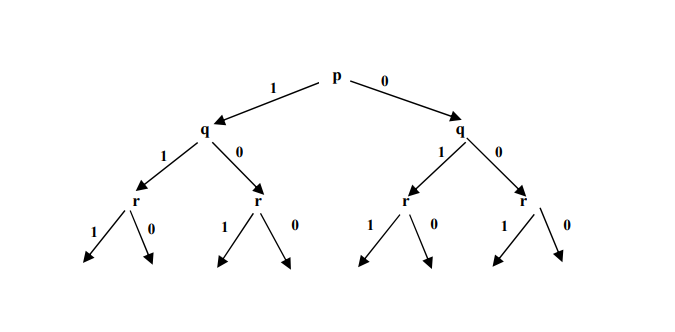
\includegraphics[width=0.8\textwidth]{Graphics/arboldp.png}
    \caption{Posible espacio de búsqueda de una FNC}
    \label{fig:arbol DP}
\end{figure}

\subsection{Davis-Putnam-Logemann-Loveland (DPLL)}
El algoritmo Davis-Putnam-Logemann-Lovelans (DPLL) aplica las mismas bases que DP, excepto que resuelve el problema de la memoria exponencial al realizar un \textit{backtrack} cronológico (al nivel anterior de decisión) en el árbol de asignaciones una vez encontrada una ``cláusula de conflicto''\footnote{Se denomina cláusula de conflicto a aquella cláusula cuyos literales evaluaron a 0 tras una asignación.}. Con este método, DPLL utiliza una estrategia \textit{``lazy''} para generar el árbol, dado que antes de ramificarse (otorgar un valor a una variable) verifica que no haya conflictos, garantizando que las asiganaciones válidas para la fórmula de entrada se encuentren en las hojas del árbol de decisión. Obsérvese que si un conflicto se produce en el nivel de decisión 0 y ambos valores para la variable ya han sido examinados, entonces se concluye que la fórmula es insatisfacible. Este proceso realizado por DPLL se denomina ramificación + propagación unitaria + retroceso.

Cabe destacar que DPLL tiene una etapa de preprocesamiento de la FNC, sobre la cual se aplican leyes de la Lógica Proposicional, así como se eliminan cláusulas redundantes mediante la aplicación de la subsunción de cláusulas\footnote{Sean $C$ y $C'$, cláusulas de una FNC; si $C' \subseteq C$, entonces se elimina $C'$ de la FNC.}. 

Obsérvese el siguiente ejemplo:

Sea la FNC:

\begin{equation*}
\{\{\neg p,\neg q\},\{\neg p, \neg q\},\{\neg p,q,\neg r\},\{\neg p,r,s\},\{p,s\}\}
\end{equation*}

Simplificando mediante la Ley de Absorción:

\begin{equation*}
\{\{\neg p,\neg q\},\{\neg p,q,\neg r\},\{\neg p,r,s\},\{p,s\}\}
\end{equation*}

Eliminando el literal puro $s$:

\begin{equation*}
\{\{\neg p,\neg q\},\{\neg p,q,\neg r\}\}
\end{equation*}

Ramificando: $p=1$

\begin{equation*}
\{\{\neg q\},\{q,\neg r\}\}
\end{equation*}

Aplicando PU:

\begin{equation*}
\{\{\neg q\},\{q,\neg r\}\}
\end{equation*}

Aplicando PU:

\begin{equation*}
\{\neg r\}
\end{equation*}

\begin{equation*}
\emptyset
\end{equation*}


Luego la FNC es satisfacible.

No obstante la reducción del espacio de memoria de DPLL respecto a DP, aún quedan problemas fundamentales: selección de variables, \textit{backtrack} cronológico y selección de cláusulas unitarias.

En primer lugar la selección de la variable a asignar un valor influye en la ``forma'' que tomará el espacio de búsqueda, por lo que malas decisiones en este sentido conllevan a caminos más largos en la búsqueda de una solución. Análogamente se gana en eficiencia considerando heurísticas en la selección de variables. (poner ejemplo)

En segundo lugar, el \textit{backtrack} cronológico a partir de un conflicto obliga a explorar el resto de las posibles asignaciones de las variables en niveles anterirores, potencialmente, de forma innecesaria, sobre todo para aquellos casos donde la asignación causante del conflicto se encuentre a $k$ niveles de distancia del nivel del conflicto. Además, DPLL no aprovecha las cláusulas que han resultado conflictos, es decir, no aprende de ellas, por lo que es vulnerable a cometer el mismo error (mismo patrón incorrecto de asignaciones para las variables involucradas en el conflicto). Esto lo hace susceptible a repetir errores de forma recurrente.

Finalmente, el problema de selección de cláusulas unitarias, influye también en la eficiencia del algoritmo. Se puede decir que guarda relacón con la estrategia de selección de variables.

\section{CDCL}
CDCL es una mejora que se le añadió al algoritmo DPLL con el objetivo de erradicar el problema del retroceso (\textit{backtrack}) cronológico, una vez encontrada una cláusula de conflicto (todos sus literales evalúan 0).

El retroceso cronológico consiste en recorrer el árbol de decisión (estructura propia del algoritmo DPLL que se forma al asignarle valores a las variables) retrocediendo de a 1 por cada nivel, probando todos los valores de cada variable hasta encontrar la asignación causante del conflicto. Esta búsqueda es ineficiente dado que, además de analizar casos innecesarios, vuelve a cometer el mismo error (potencialmente realiza la misma combinación de asignaciones) generando búsquedas redundantes.
Para solucionar este problema, CDCL crea un grafo dirigido y acíclico que permite guardar el historial de asignaciones de cada variable. En dicho grafo, los nodos son las variables y los arcos constituyen la causa de la asignación de dicha variable: la cláusula a la que pertenece, si fue asignada por propagación unitaria, y null para variables asignadas por decisión. El grafo también contiene 2 metadatos: el valor asignado a cada variable (0 o 1), y el nivel de decisión en el que se asignó (los diferentes niveles de decisión están marcados por la asignación de valores por decisión). Cabe destacar que la dirección de los arcos en el grafo va desde las variables de decisión hacia aquellas que, en el mismo nivel, tuvieron que forzar su valor por propagación unitaria. En el caso de una nueva variable de decisión, se crea un nuevo arco con valor nulo desde la variable asignada por decisión en el nivel anterior, hasta la nueva variable.

Cuando una cláusula resulta ser de conflicto (sus literales evaluaron 0), CDCL crea un nuevo nodo en el grafo que representa dicho conflicto, para comenzar con su análisis.
Este análisis busca en el grafo la asignación causante del conflicto, para retroceder justo hacia ese punto y realizar un \textit{backjump} en lugar de un retroceso cronológico, como en DPLL. Asimismo, con este análisis CDCL busca conformar una cláusula (cláusula aprendida) que represente la combinación de asignación de valores que condujo a dicho conflicto, para incluirla en la base de datos de las cláusulas de la FNC y evitar cometer el mismo error en iteraciones futuras. El punto escogido para realizar el \textit{backjump} es conocido como primer punto de implicación único (\textit{First-UIP} por sus siglas en inglés). Este punto, será aquel literal que en la cláusula aprendida, posea el más alto nivel de decisión, diferente del actual.

Es necesario enfatizar en el hecho de que la cláusula aprendida debe contener únicamente 1 literal cuyo valor haya sido asignado en el nivel de decisión actual. En caso de haber más de uno, CDCL recorre el grafo en busca de la cláusula que causó la asignación de una de estas variables y aplica el Principio de Resolución entre esta y la cláusula aprendida hasta el momento. La cláusula resultante pasará a ser la nueva cláusula aprendida. El proceso se repetirá hasta que la cláusula aprendida contenga solo un literal cuyo valor fue asignado en el nivel de decisión actual.

En caso de que el nivel del \textit{backjump} sea el nivel 0, CDCL considera la FNC como insatisfacible.

(poner ejemplos) INSERTAR C\`ODIGO

\section{DLIS}
La heurística Dynamic Largest Individual Sum (DLIS) para selección de variables, es uno de los métodos aproximados que pueden integrarse en un CDCL SAT \textit{solver} con el objetivo de aumentar la eficiencia al asignar un valor a una variable en cada nivel de decisión.

DLIS lleva un contador por cada variable que indica el número máximo que clásulas insatisfechas que pueden resolverse al asignar uno de los dos valores (0 o 1). Es decir, dada una variable $x$, se calcula la cantidad de cláusulas insatisfechas en las que aparece el literal $x$ y su complementario $\neg x$. Sea $dlis(x)$ la mayor cantidad de cláusulas que $x$ puede satisfacer, y $count_pos(x)$ y $count_neg(x)$ la cantidad de veces que aparece el literal positivo y negativo, repectivamente, en cláusulas aún sin resolver; luego:

\begin{equation*}
dlis(x)=max(count_pos(x), count_neg(x))
\end{equation*}

Teniendo en cuenta este cálcula la próxima variable a asignar será:
\begin{equation*}
x_k \mid dlis(x_k)=max(dlis(x_i)), i \in [1,n]
\end{equation*}

donde $n$ es la cantidad de variables de la FNC.

Obsétvese que si $count_pos(x_k) > count_neg(x_k)$ entonces $x_k$ tomará como valor 1, y 0 en caso contrario, puesto que el objetivo es satisfacer dichas cláusulas. Téngase en cuenta que el cálculo se le aplica a las variables que aún no han sido asignadas, además de solo tenerse en cuenta aquellos valores que aún no han sido explorados para una misma variable en el actual nivel de decisión.

% % % % % % INSERTAR CóDIGO ACá % % % % % % % %

Con esta estrategia DLIS busca satisfacer en una misma asignación la mayor cantidad de cláusulas posibles, sin embargo, esta estrategia resulta costosa en instancias grandes $O(n)$ por cada nivel de decisión.

\section{VSIDS}
Por su parte, la heurística Variable State Independent Decaying Sum (VSIDS) prioriza asignarle valores aquellas variables que hayan estado en conflictos recientes. Para ello, VSIDS lleva un \textit{score} por cada literal $l$ (no por cada variable) que aumenta cada vez que aparezcan en clásulas aprendidas de conflictos. Además, para evitar que literales que hayan pertenecido a conflictos pasados y no recientes sean tenidos en cuenta por encima de los más actuales, cada cierta cantidad $T$ de conflictos se multiplica los \textit{scores} de cada literal por $\alpha$, donde $0 < \alpha < 1$ (usualmente $\alpha = 0.95$). Integrado con CDCL, VSIDS se comportaría de la siguiente forma:
\begin{enumerate}
    \item Procede el algoritmo CDCL.
    \item Si ocurre un conflicto, se añade la cláusula aprendida $\mathbf{C_{learn}}$. Luego, por cada literal $l$ tal que $l \in \mathbf{C_{learn}}$ se tiene que $score(l) += \delta$, donde $\delta$ es el incremento.
    \item Si ocurre el conflicto $T$-ésimo, entonces $\delta = \delta \cdot \alpha$ con $0 < \alpha < 1$.
    \item Si no ocurre un conflicto, se seleccionará según VSIDS la variable $v$ si $score(l_v) = \max(score(l_i))$ para todo $i$ tal que $1 \leq i \leq 2n$, con $n$ cantidad de variables. Si $l_v$ es positivo, entonces $v$ tomará valor 1, y 0 en caso contrario.
\end{enumerate}


% % % % INSERTAR CóDIGO ACá % % % %

\section{Reinicio (\textit{restart})}
Las estrategias de reinicio buscan no estancarse en espacios locales de búsqueda mediante un ``reinicio'' del árbol de decisión, es decir, eliminan todas las asignaciones realizadas hasta el momento y vuelven a empezar, pero manteniendo en la FNC las cláusulas aprendidas producto de CDCL, y los datos extras como \textit{scores} de los literales que hayan aportado las heurísticas de selección de variables.

Existen varios criterios para realizar los \textit{restarts}:
\begin{enumerate}
\item Fijo: se reinicia cada $k$ conflictos fijos.
\item Geométrico: cada intervalo $r_i$ crece como un secuencia geométrica de la siguiente forma: $r_0 = b; r_i = \alpha \cdot r_{i-1} \mid \alpha > 1$. Es importante definir bien el valor de $\alpha$ pues si este es muy grande los reinicios serán muy espaciados, y si es muy pequeño habrá una sobrecarga de \textit{restarts}.
\item Luby: Este reinicio se basa en la secuencia de Luby (1,1,2,1,1,2,4,1,1,2,…), obteniéndose que $r_i = b \cdot Luby(i)$, donde $r_i$ constituye el i-ésimo \textit{restart}, y $b$ es un parámetro de intervalo.
\item \textit{Glucose-style (LBD-based)}: esta estrategia está basada en el cálculo Literal Block Distance (LBD) que consiste en, dada una cláusula aprendida, contar la cantidad de niveles de decisión diferentes a los que pertenecen cada uno de sus literales. Es decir, dada una cláusula aprendida $C_{learm}$ se tiene que $LBD(C_{learn}) = \|\{level(l)\: l \in C_{learn} \}\|$. LBD busca medir la calidad de una cláusula a partir de la diversidad de niveles de decisión en una cláusula, planteando que mientras menor sea este número las variables implicadas en el conflicto estarán más cerca en el árbol de decisión, por ende más relacionadas, luego más útil la cláusula. Por tanto, a menor LBD, mayor calidad de cláusula. Ahora, la estrategia de reinicio \textit{Glucose-style} haya dos promedios de LBD para una ventana ``rápida'' (usualmente 50 o 100 últimos conflictos) y una ventana ``lenta'' (usualmente 1000 últimos confilctos)de cantidad de conflictos. Estas dos cantidades se dividen de la siguiente forma: sean $\mu_r$ promedio de LBD en la ventana rápida de últimos conflictos, y $\mu_l$ su homólogo para la ventana lenta; sea, además, $T > 1$ umbral de decisión, entonces \textit{Glucose-style} realiza la comparación $\dfrac{\mu_r}{\mu_l} > T$, y si esta resulta verdadera entonces procede con el reinicio. Esta estrategia sugiere que si el promedio de LBD en cláusulas aprendidas recientes supera significativamente al de cláusulas más antiguas, el algoritmo estaría estancado en espacios locales de búsqueda infructíferos.
\end{enumerate}

% % % %INSERTAR CóDIGO ACá, PREFERIBLEMENTE POR CADA ESTRATEGIA % % % %

\section{Selección de cláusulas unitarias}

Una de las estrategias más usadas actualmente es \textit{Two Watched Literals (TWL)}. Esta tiene por objetivo evitar el recorrido de todas las cláusulas en el momento de realizar la propagación unitaria mediante la ``vigilancia'' de dos literales $l_1$ y $l_2$ por cada cláusula. Si durante el algoritmo tanto $l_1$ como $l_2$ no han sidp evaluados, pues no es necesario revisar dicha cláusula dado que no es unitaria ni de conflicto. En cambio, si alguno ha sido asignado a 0 se busca en cada cláusula otro literal para sustituirlo y, de no ser posible implicaría que la cláusula es unitaria (asumiendo que el otro literal vigilado no tiene valor). Si ambos literales son evaluados a 0, entonces la cláusula es de conflicto. Esta estrategia reduce grandemente el costo de recorrer cada cláusula en cada nivel de asignación.

% % % %INSERTAR CóDIGO % % % %